
%%% Local Variables: 
%%% mode: latex
%%% TeX-master: t
%%% End: 

\chapter{解码器性能优化实验结果}
\label{cha:optresultandanalysis}

本章主要介绍对解码器优化结果的测试方法及结果。首先说明了生成测试数据的过程,然后使用这些数据对优化前后的解码器进行测试,对比结果。

\section{测试数据的生成}
\label{sec:optresultsgeneration}

测试数据采用\refsec{sec:introtojmvc}中提到的参考软件JMVC和ffmpeg\footnote{\url{http://www.ffmpeg.org/}}配合生成。ffmpeg用来将多种格式(如AVI、MP4)的视频转换为YUV格式。JMVC中的H264AVCEncoderLibTestStatic用来对N路YUV视频压缩成H.264流,MVCBitStreamAssemblerStatic用来将多路H.264打包成一个MVC视频流。我们测试的视频分为3类:一路、两路和八路的多视点视频。他们的生成方法较为类似,我们以八路视频为例,说明生成的具体方法:
\begin{enumerate}
\item 首先要编写一个描述视频压缩参数的配置文件,我们实际使用的配置文件之一见\autoref{lst:mvccfg}。其中比较关键的项为
\begin{description}
\item[InputFile] 输入的文件名格式,golf1表示输入的各路视频为golf1\_0.yuv、golf1\_1.yuv、\dots、golf1\_7.yuv。
\item[OutputFile] 输出的文件名格式,与InputFile类似。输出的文件扩展名为.264。
\item[SourceWidth] 待编码的视频水平分辨率\footnote{由于YUV视频的内容只是视频每一帧的实际数据,不像我们常使用的一些被包装在容器中的视频格式,并没有存储视频的分辨率、帧率等参数。},如320。
\item[SourceHeight] 待编码视频的垂直分辨率,如240。
\item[FrameRate] 待编码视频的帧率,如30.0。
\item[FramesToBeEncoded] 从YUV文件的第一帧算起,一共需要编码的帧数,如623。
\item[GOPSize] 参考结构中的GOP大小的上限,如4。对这个参数的设置影响参考结构的复杂程度。
\item[NumViewsMinusOne] 编码视频的路数减1,如7。
\item[ViewOrder] 各路视频的编码顺序,如0-2-1-4-3-6-5-7。
\end{description}
其他还有一些对每一路视频的参考结构的限定,我们采用与JMVC的demo中相同的参考结构。
\item 有了上述的配置文件MVC.cfg\footnote{文件名可以取任意合法的文件名,对扩展名没有要求。}之后就可以使用如下的命令来编码了\\H264AVCEncoderLibTestStatic.exe -vf MVC.cfg 0\\这个命令使用MVC.cfg中定义的参数对View 0进行编码。想要编码全部8路视频需要严格按照MVC.cfg中ViewOrder定义的顺序进行编码。
\item 编码生成了8个H.264码流之后,我们需要将其打包成一个文件。MVCBitStreamAssemblerStatic就是这样的一个packer,它也需要一个配置文件,样例见\autoref{lst:assemblercfg}。其中定义了输入输出的文件名以及视频的路数。这里对输入文件的列举顺序没有要求,只要文件与视角对应即可。使用如下命令可以将码流打包:\\MVCBitStreamAssemblerStatic.exe -vf assembler.cfg
\item 由于JMVC的编码器性能极其低下\footnote{我们编码这个分辨率为$320\times 240$,一共623帧的golf623.mvc总共耗费了近四个小时。},我们推荐使用批处理来依次执行这些编码命令,免去每隔十几或几十分钟需要人工进行下一步编码命令的输入操作。一个批处理的样例见\autoref{lst:batchEncode}。
\end{enumerate}

我们能够在网上获取的用于研究的YUV格式多视点样例视频片段大多是QVGA的分辨率,这一方面由于在我们进行多视点视频解码器优化之前,已有的编解码器性能很差;另一方面是由于YUV格式对数据几乎没有压缩,需要大量的存储空间\footnote{我们测试用的$1280\times 720$的两路视频,仅仅两秒左右(65帧)就需要$85.7$MB$\times2$的空间。}。我们的测试目标针对的是分辨率至少为$720\times 576$的视频,这样的YUV源很难获得,需要自己生成。

值得庆幸的是,NVIDIA为了推广其3D产品,在网站上提供了几段高清的两路视频片段。我们使用ffmpeg将其中分辨率为$1440\times 1080$的一个WMV视频转换成两路独立的YUV文件。
\begin{enumerate}
\item 我们首先使用了MPEG Streamclip\footnote{\url{http://www.squared5.com/}}将这个$2880\times 1080$的WMV裁剪成左右两个$1440\times 1080$的部分。分别存为left\_1440x1080.mp4和right\_1440x1080.mp4。
\item 使用如下命令将视频转为目标分辨率(如$1280\times 720$)的YUV视频:\\
ffmpeg.exe -y -i left\_1440x1080.mp4 -ss 41 -vframes 65 -s 1280x720 dualtest\_1280x720\_65f\_0.yuv\\
ffmpeg.exe -y -i right\_1440x1080.mp4 -ss 41 -vframes 65 -s 1280x720 dualtest\_1280x720\_65f\_1.yuv\\
这里我们转换了从第41帧起的65帧画面。
\item 对这两个生成的YUV视频用前文提到的JMVC编码的方法就可以编码并打包成两路的MVC测试视频了。
\end{enumerate}

我们还使用了一段电影$\mathit{Avatar}$的花絮$\mathit{The\ World\ of\ Pandora}$中的片段生成一路的测试视频。

使用如下命令生成YUV文件:

ffmpeg.exe -y -i The\_World\_of\_Pandora.mov -ss 15 -vframes 65 -s 1280x720 singletest\_1280x720\_65f\_0.yuv

再用JMVC编码打包成一路MVC视频。

至此我们生成了全部用于测试的MVC视频,进行测试用到的所有视频的属性如\autoref{tab:testclips}所示:

\begin{table}[htbp]
  \centering
  \begin{minipage}[t]{\linewidth}
  \caption{性能测试中使用的所有视频一览}
  \label{tab:testclips}
  \centering
    \begin{tabular}{lrrr}
    \addlinespace
    \toprule[1.5pt]
    \textbf{Clip Name} & \textbf{Resolution} & \textbf{Num of Frames} & \textbf{Num of Ways} \\
    \midrule[1pt]
    dual144		& $176\times 144$	& 65	& 2 \\
    dual288		& $352\times 288$	& 65	& 2 \\
    dual576		& $720\times 576$	& 65	& 2 \\
    dual720		& $1280\times 720$	& 65	& 2 \\
    golf25		& $320\times 240$	& 25	& 8 \\
    golf25dual	& $320\times 240$	& 25	& 2 \\
    golf623		& $320\times 240$	& 623	& 8 \\
    race81		& $320\times 240$	& 81	& 8 \\
    single144	& $176\times 144$	& 65	& 1 \\
    single288	& $352\times 288$	& 65	& 1 \\
    single576	& $720\times 576$	& 65	& 1 \\
    single720	& $1280\times 720$	& 65	& 1 \\
    \bottomrule[1.5pt]
    \end{tabular}
  \end{minipage}
\end{table}

\section{实验结果及说明}
\label{sec:optresult}

我们用解码器解码\autoref{tab:testclips}中地每一个视频。优化前的基准性能见\autoref{tab:desktopBaseline},Visual Studio自带的编译器编译出的解码器的性能见\autoref{tab:desktopMS},ICC编译出来的解码器性能见\autoref{tab:desktopICC}。

参考《$\LaTeX$ and and the GNUPLOT Plotting Program》\cite{kotz1991latex}和《gnuplot 4.4: An Interactive Plotting Program》\cite{williams2009interactive},用gnuplot\footnote{\url{http://www.gnuplot.info/}}对其中部分数据制图。
% 对比
% 8-way golf25 golf623 race81
% 2-way golf25dual Prof_Bullinger_720x576_65f_dual

% 单核优化结果,对不同分辨率和路数
% singletest dualtest

% 多核优化结果,对不同分辨率和路数
% singletest dualtest golf25dual golf25 golf623 race81 Prof_Bullinger_720x576_65f_dual

% 不同平台cpu上的测试 intel core 2 duo T7200
% singletest dualtest golf25dual golf25 golf623 race81 Prof_Bullinger_720x576_65f_dual

\begin{figure}[htbp]
\begin{center}
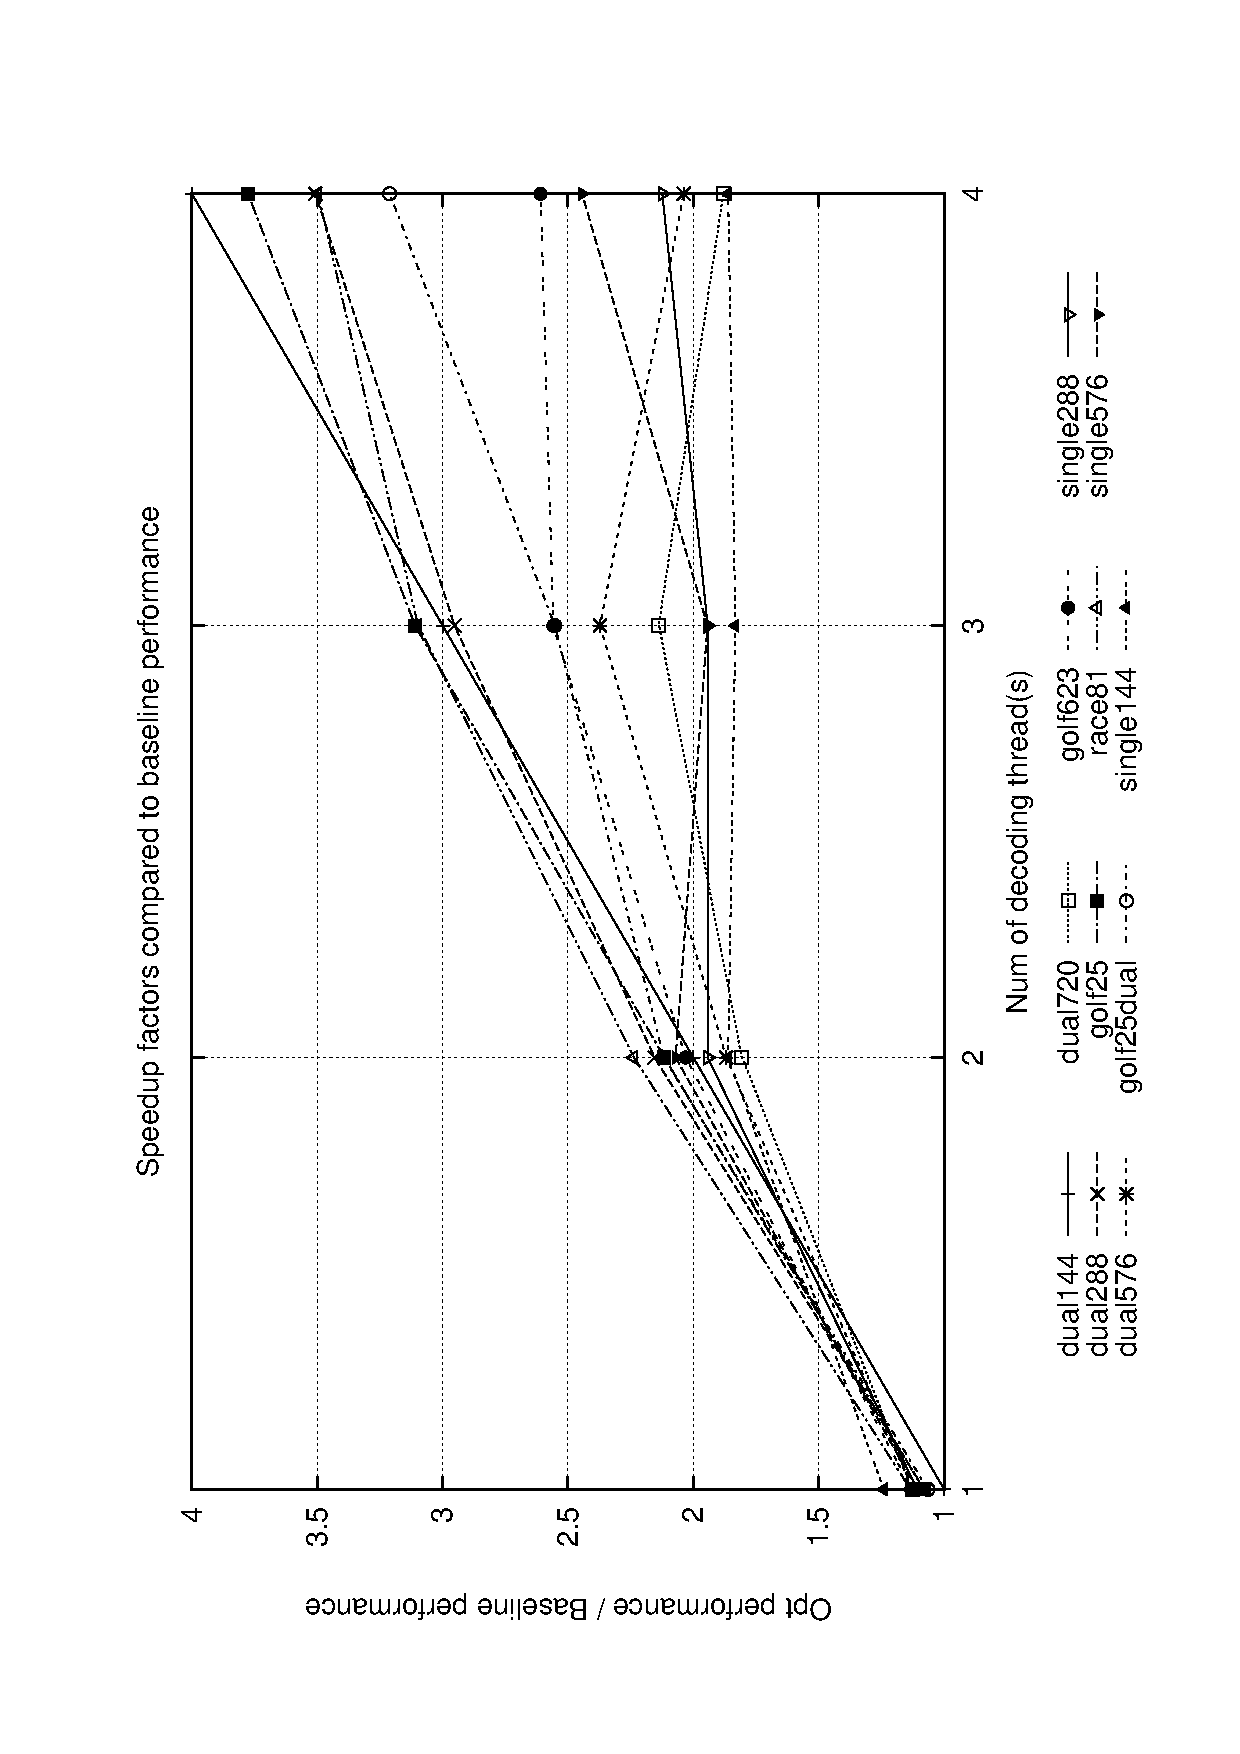
\includegraphics[height=\textwidth,angle=-90]{speedupMS}
\caption{解码不同视频的加速比(使用MS编译器)}
\label{fig:speedupMS}
\end{center}
\end{figure}


\begin{figure}[htbp]
\begin{center}
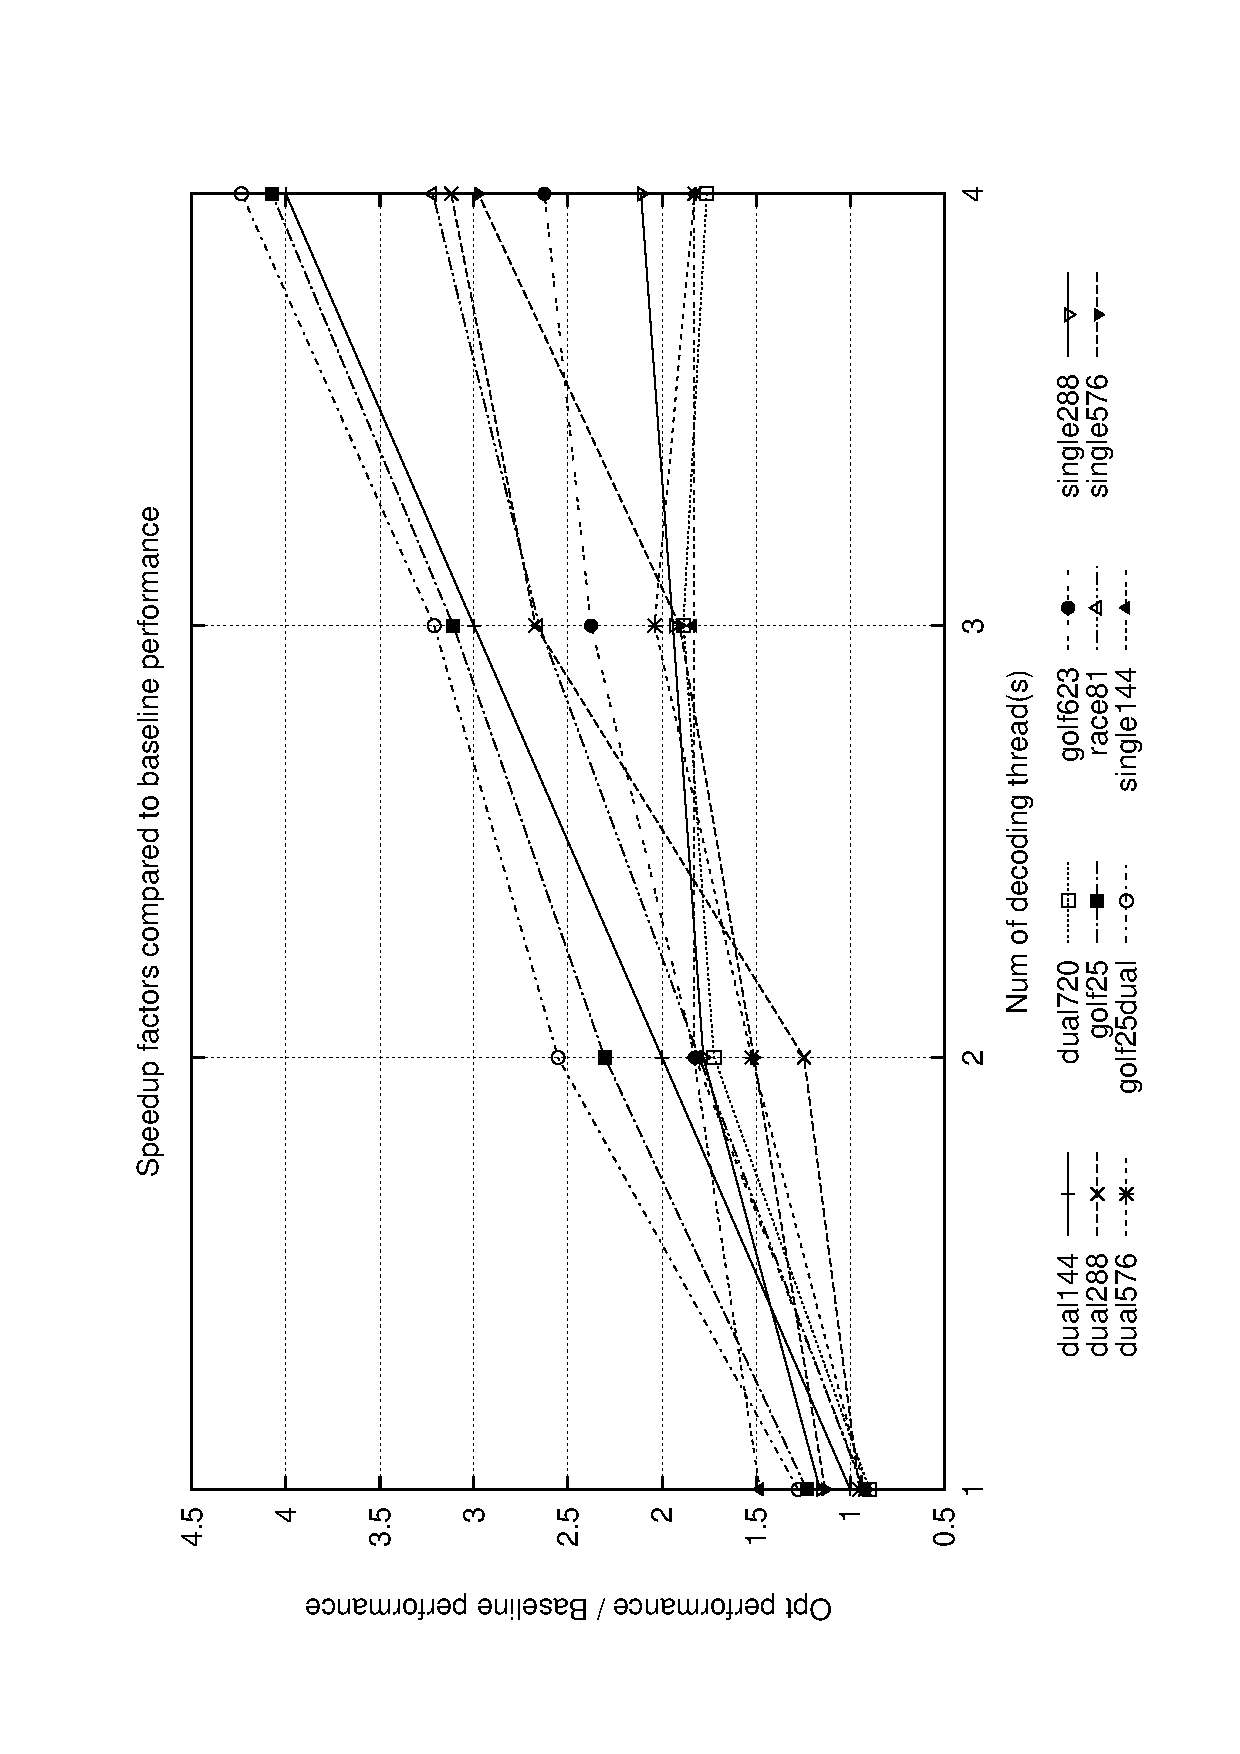
\includegraphics[height=\textwidth,angle=-90]{speedupICC}
\caption{解码不同视频的加速比(使用ICC编译器)}
\label{fig:speedupICC}
\end{center}
\end{figure}

经过优化后的解码器支持大于1的解码线程数。用Visual Studio内置的微软编译器编译的解码器用1到4个线程解码各个测试样例的性能与优化前的基准性能相比的加速比如\autoref{fig:speedupMS}所示。用ICC编译器编译的解码器的加速比如\autoref{fig:speedupICC}所示。更清晰的版本附在在本章末尾的\autoref{fig:speedupMS2}和\autoref{fig:speedupICC2}。

可以看出,几条折线的趋势都证明增加线程数能够加快解码速度,而几条折线在线程数为3和4时的变化又有所不同:
\begin{itemize}
\item dual144的加速比正好为线程数,这是一个巧合。不过也能部分说明当视频的并行性足够时,增加的线程资源能够被充分利用。
\item golf25、golf25dual、dual288和race81这四个视频也能充分利用额外的资源。
\item single144、single288、single576、single720这些单路的视频加速比都没有超2.6,这是由于一路视频的参考结构比较简单,没有视角间的参考。调度器很难安排出能够并行处理的大于2个任务。
\item golf623的加速比低于预期,我们推测的原因时编码时的GOPSize设成4对于8路视频偏小了,造成并行程度不够。
\end{itemize}


对部分测试视频的解码帧率如\autoref{fig:viewerfps}。这里计算的帧率是同时解码N路时的帧率,也就是观看者实际看到的等效帧率。对两路视频而言,要达到30fps的等效帧率,必须能够实际解码速率达到60fps。

从图中可以看到,对于实验目标针对的$720\times 576$的两路视频,只要线程数超过一个,就已经达到并超过了设定的实验目标。

\begin{figure}[htbp]
\begin{center}
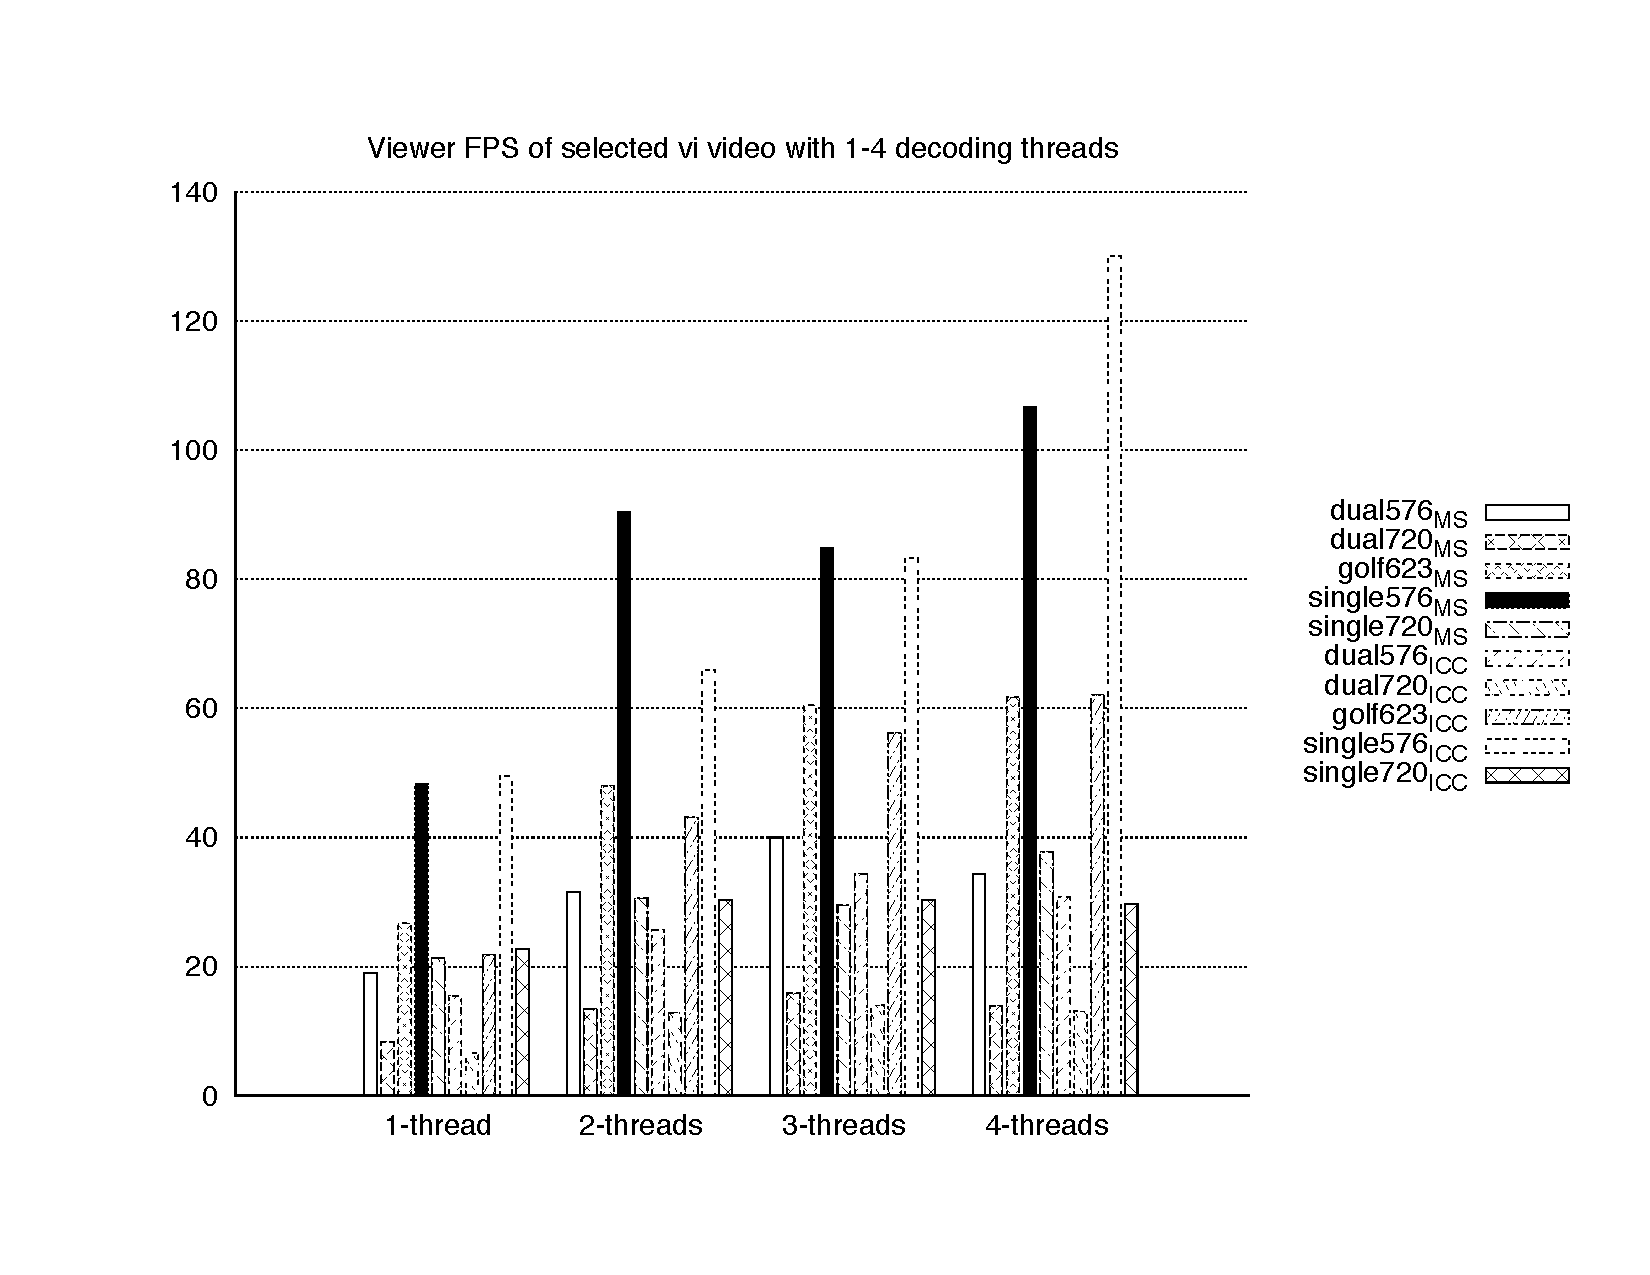
\includegraphics[width=\textwidth]{viewerfps}
\caption{部分视频解码的等效帧率}
\label{fig:viewerfps}
\end{center}
\end{figure}

\section{小结}
\label{sec:sum6}

本章详细介绍了测试解码器性能的视频准备工作;比较了优化后的解码器优化前的性能提升,不同的测试视频得到了不同的结果,但是总的趋势是符合逻辑的;数据表明优化后的解码器达到了先前设定的目标。


\begin{figure}[htbp]
\begin{center}
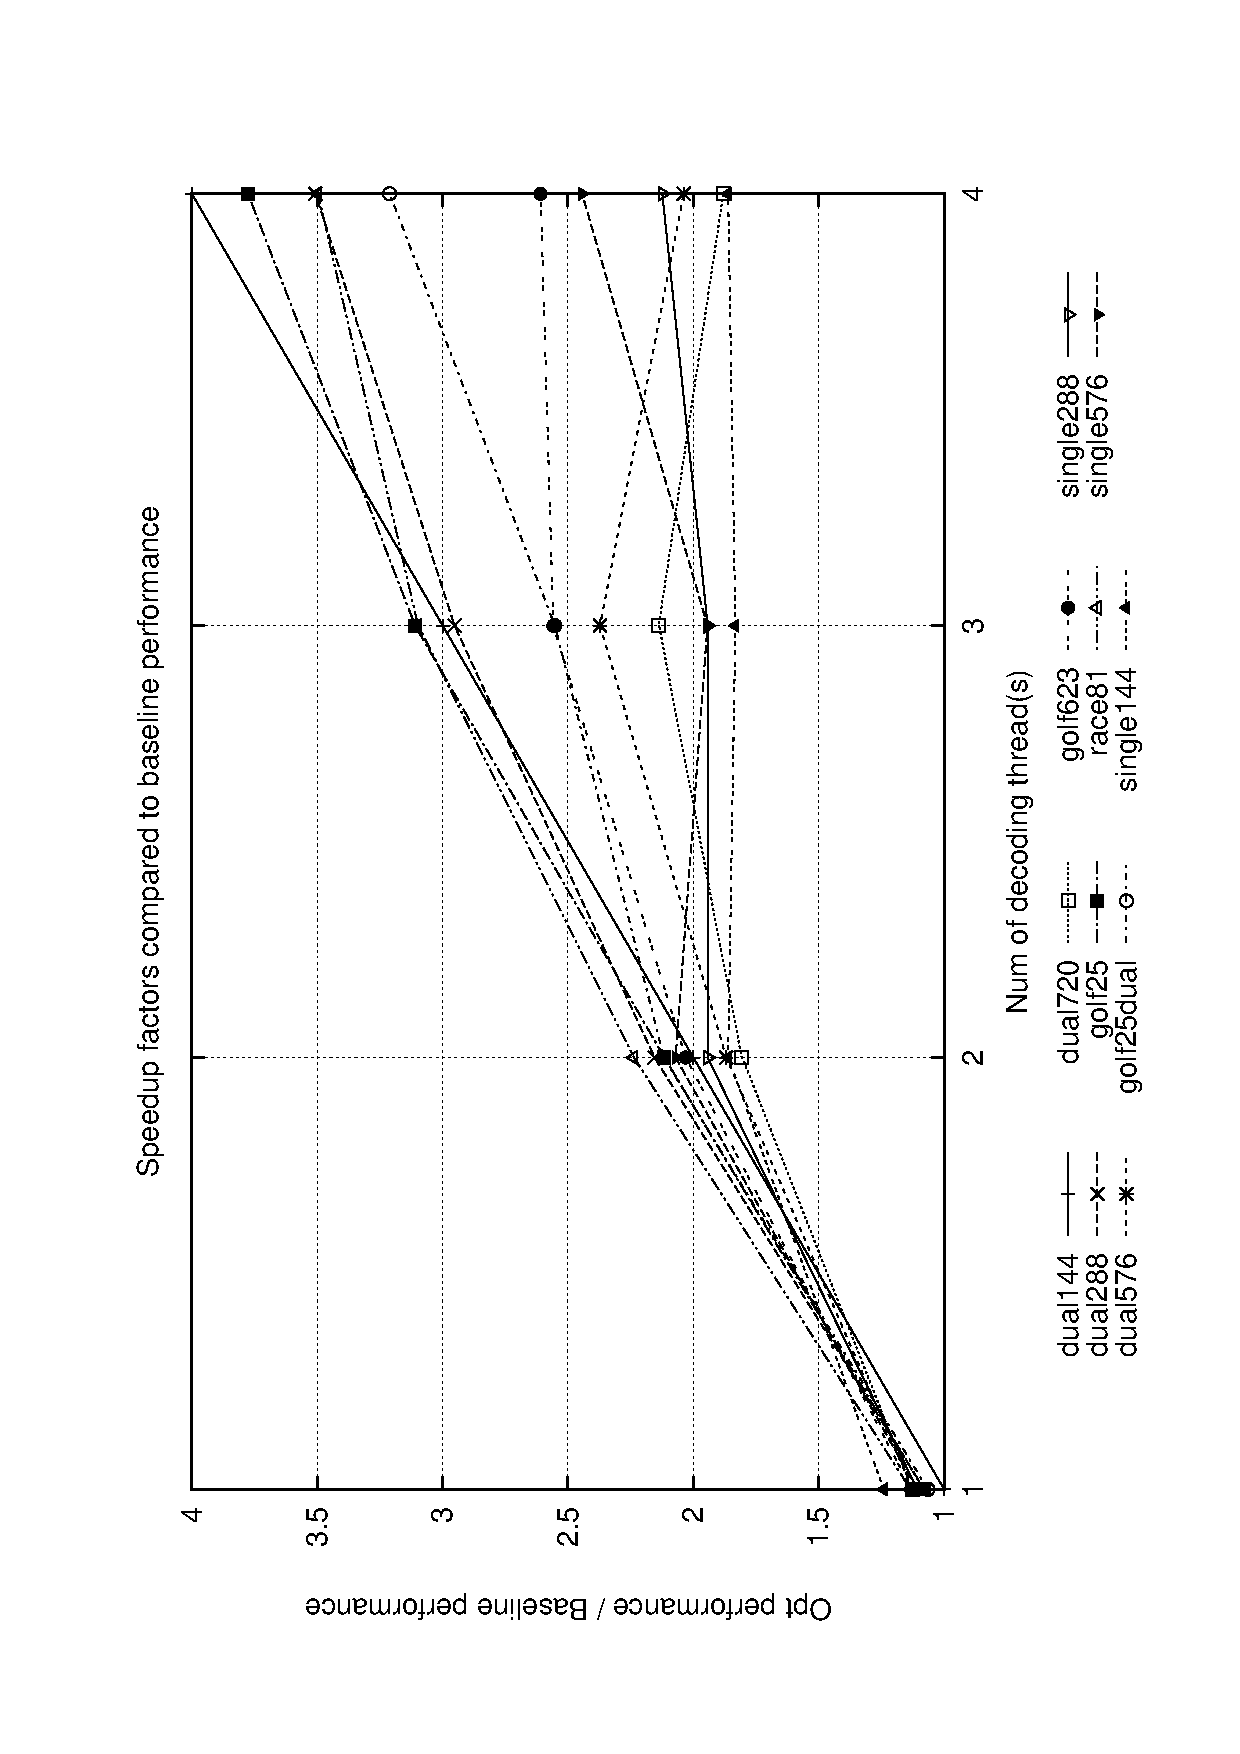
\includegraphics[width=\textwidth]{speedupMS}
\caption{解码不同视频的加速比(使用MS编译器)}
\label{fig:speedupMS2}
\end{center}
\end{figure}


\begin{figure}[htbp]
\begin{center}
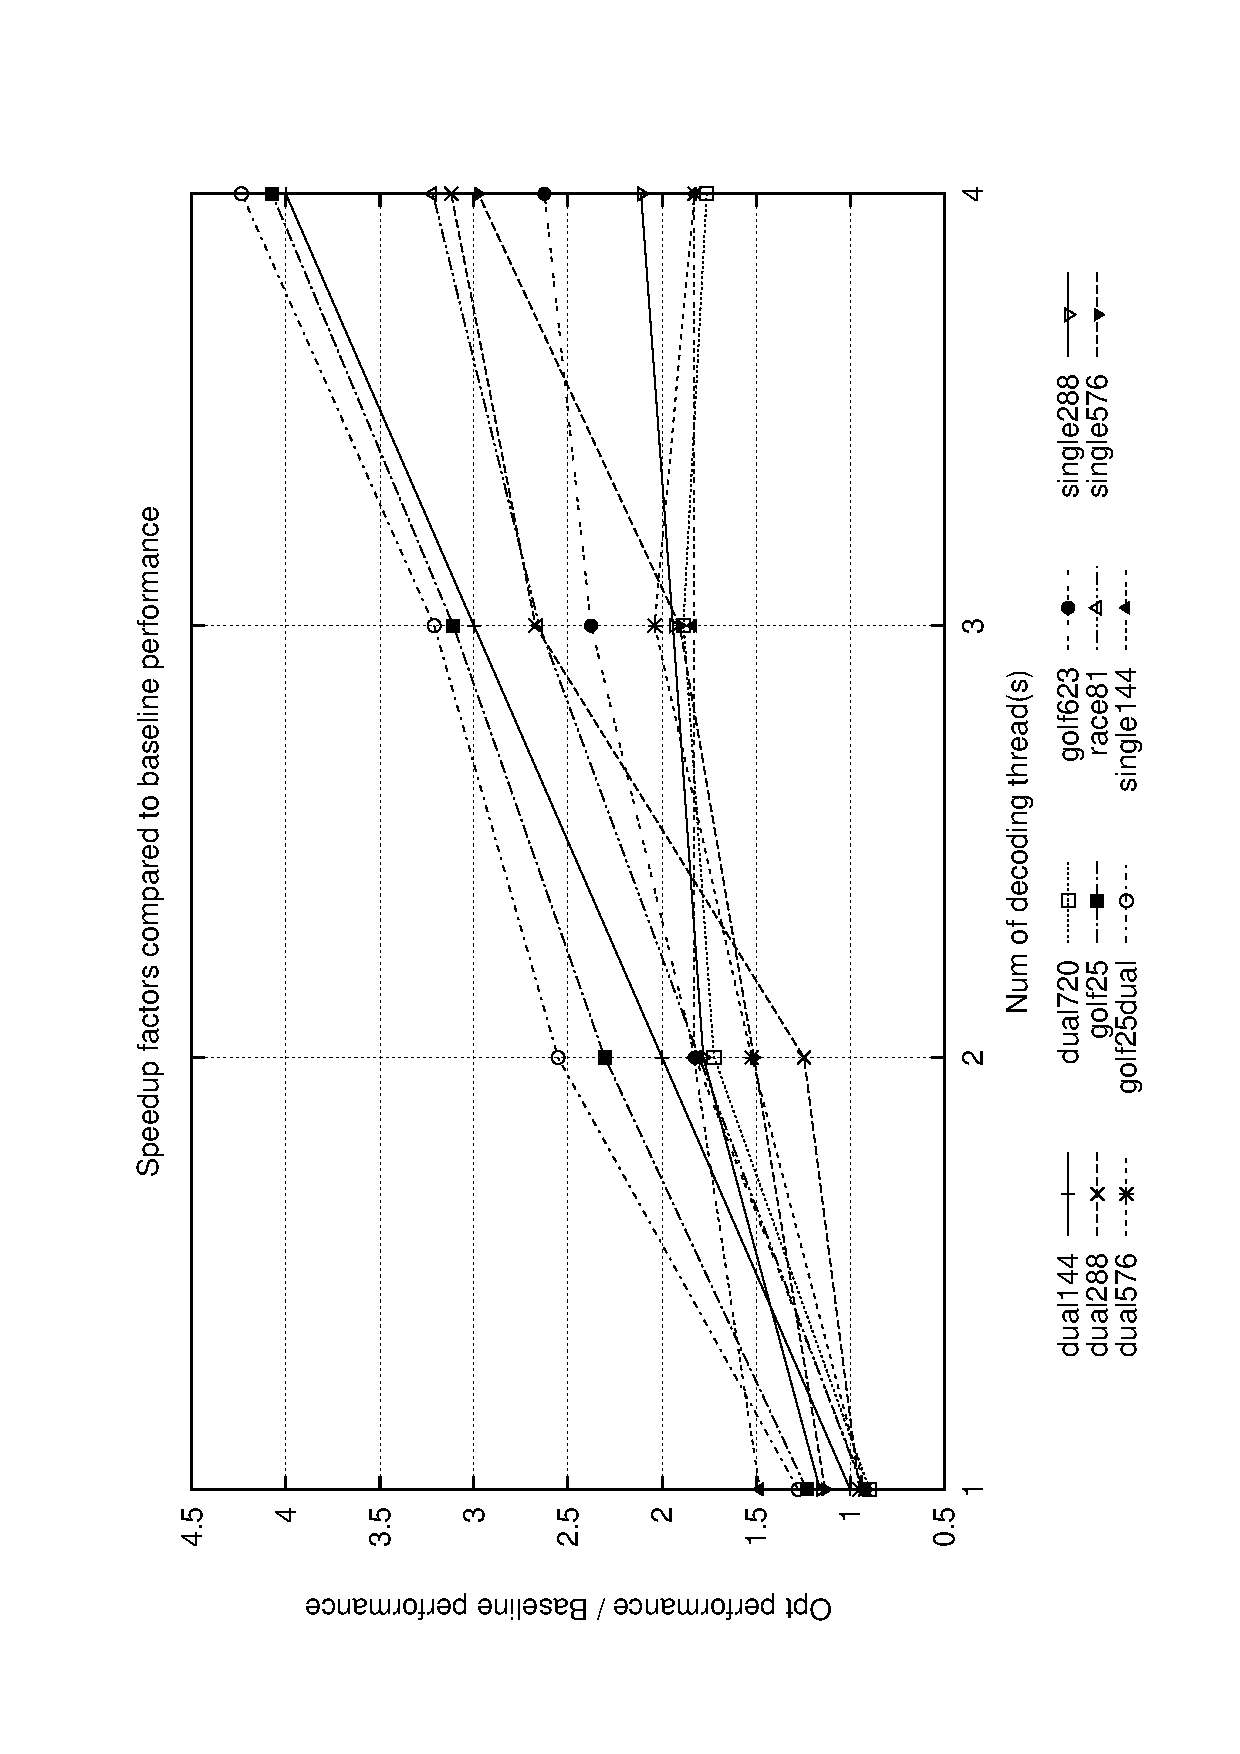
\includegraphics[width=\textwidth]{speedupICC}
\caption{解码不同视频的加速比(使用ICC编译器)}
\label{fig:speedupICC2}
\end{center}
\end{figure}


\cleardoublepage